\documentclass{article}

\usepackage{lmodern} % font
\renewcommand\familydefault{\sfdefault} % font
%\usepackage{fancyhdr} % header and footer
\usepackage[a4paper, margin=3cm]{geometry} % margin
\usepackage{mdframed} % frame
\usepackage{multicol} % multicolumn
\usepackage{graphicx} % images
\usepackage[labelformat=empty]{caption} % caption without prefix
\usepackage{flushend} % align
\usepackage{amsmath} % math
\usepackage{mathtools} % rcases
\usepackage{amsfonts} % math
\usepackage{listings} % code
\usepackage{xcolor} % color
\usepackage{amssymb} % math
\usepackage{mdframed} % frame

\title{Algoritmi e Strutture Dati}
\author{Leonardo Baldo}
\date{}

\begin{document}

\maketitle
\newpage

\tableofcontents
\newpage

\section{Introduzione}
\begin{mdframed}
    \textbf{Algoritmo:} procedura che descrive tramite passi elementari come risolvere un problema (tramite un modello di computazione).
\end{mdframed}

\raggedright
Uno stesso problema può essere risolto da diversi algoritmi. Di ogni algoritmo siamo interessati a conoscere:
\begin{itemize}
    \item correttezza
    \item stabilità
    \item complessità
\end{itemize}

\subsection{Induzione}
L'induzione si struttura con:
\begin{itemize}
    \item Un caso base $P(0)$.
    \item Un'ipotesi induttiva (se vale per $P(n)$ allora vale anche per $P(n+1)$).
\end{itemize}

Matematicamente parlando significa che:
\begin{itemize}
    \item Normalmente ho una formula, per esempio $n=1$.
    \item Se vale per $n=1$, provo con $n=2$.
    \item Se funziona anche con $n=2$, vuol dire che per $P(n)$ varrà anche $P(n+1)$ e tutti i successivi.
\end{itemize}

Si ha anche un'ulteriore variante, l'induzione forte:
\begin{itemize}
    \item $U$ contiene $1$ oppure $0$.
    \item Se $U$ contiene tutti i numeri minori di nallora contiene anche $n$.
\end{itemize}

La parola "forte" è legata al fatto che questa formulazione richiede delle ipotesi apparentemente più forti e stringenti per inferire che l'insieme $U$ coincida con $N$ per ammettere un numero nell'insieme è richiesto infatti che tutti i precedenti ne faccianogià parte (e non solo il numero precedente).

\subsection{Ricorrenza}
\begin{mdframed}
    \textbf{Relazione di ricorrenza} è una formula ricorsiva che esprime il termine $n$-esimo di una successione in relazione ai precedenti.
    La relazione si dice di ordine $r$ se il termine $n$-esimo è espresso in funzione al più dei termini $(n - 1), \ldots, (n - r)$.
\end{mdframed}

\newpage
\section{Insertion Sort}
L'array viene virtualmente diviso in una parte ordinata e una non ordinata. I valori della parte non ordinata vengono prelevati e collocati nella posizione corretta della parte ordinata. \\

Caratteristiche dell'ordinamento per inserzione:
\begin{itemize}
    \item Questo algoritmo è uno dei più semplici e di semplice implementazione.
    \item Fondamentalmente, l'ordinamento per inserzione è efficiente per piccoli valori di dati
    \item L'ordinamento per inserzione è di natura adattativa, cioè è adatto a insiemi di dati già parzialmente ordinati.
\end{itemize}
Quello che sostanzialmente fa è esaminare gli elementi a coppie e ordinarli gradualmente per come si presentano.

\begin{center}
    \begin{tabular}{c}
        \\ 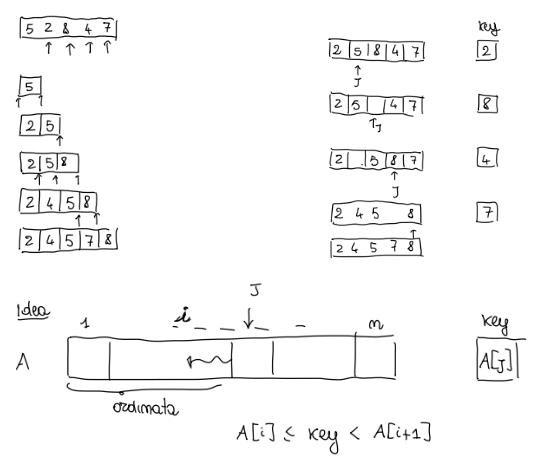
\includegraphics[width=0.5\textwidth]{image/InsertionSortExample.png} \\ \\
    \end{tabular}
\end{center}

\subsection{Pseudocodice}
\begin{mdframed}
\begin{lstlisting}[language=C]
INSERTION-SORT(A)
1   n = A.length
2   for j = 2 to n
3       key = A[j]
4       i = j - 1
5       while i > 0 and A[i] > key
6           A[i + 1] = A[i]
7           i = i - 1
8       A[i + 1] = key
\end{lstlisting}
\end{mdframed}

\subsection{Correttezza}
Definiamo i seguenti passi per $A$ da indice $1$ ad indice $j-1$
\paragraph{Inizializzazione:} $j=2, A[1,1]$ ordinato
\paragraph{Mantenimento:} inserisce $A[j]$ in $A[1 \; ... \; j-1]$ ordinato
\paragraph{Cancellazione:} $j=n+1$

\newpage
\section{Merge Sort}

Adotta l'approccio divide et impera, quindi:
\begin{itemize}
    \item divide: prende il problema originale e lo divide in problemi più piccoli.
    \item impera: ricorsivamente, risolve i sottoproblemi; se abbastanza piccolo, si risolve subito.
    \item combina: le soluzioni di $P_1$,...,$P_k$ si combinano in una soluzionedi $P$.
\end{itemize}

Quindi, mergesort adotta i seguenti passi:
\begin{itemize}
    \item dividere l'array in due parti
    \item ordina i sottoarray
    \item fonde i sottoarray ordinati
\end{itemize}

\begin{center}
    \begin{tabular}{c}
        \\ 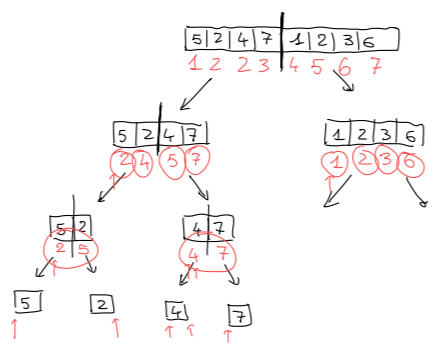
\includegraphics[width=0.6\textwidth]{image/MergeSortExample.png} \\ \\
    \end{tabular}
\end{center}

\newpage
\subsection{Pseudocodice}
\begin{mdframed}
\begin{lstlisting}[language=C]
MERGE-SORT(A,p,r)
1   if p < r
2       q = (p+r)/2
3       MERGE-SORT(A,p,q)
4       MERGE-SORT(A,q+1,r)
5       MERGE(A,p,q,r)
\end{lstlisting}
\end{mdframed}
\begin{mdframed}
\begin{lstlisting}[language=C]
MERGE(A,p,q,r)
1   n1 = q - p + 1
2   n2 = r - q
3   for i = 1 to n1
4       L[i] = A[p+i-1]
5   for j = 1 to n2
6       R[j] = A[q+j]
7   L[n1+1] = R[n2+1] = infinity
8   i = j = 1
9   for k = p to r
10      if L[i] <= R[j]
11          A[k] = L[i]
12          i = i + 1
13      else // L[i] > R[j]
14          A[k] = R[j]
15          j = j + 1
\end{lstlisting}
\end{mdframed}

\subsection{Complessità}
$A[p, ..., k-1]$ contiene $L[1, ..., i-1]$ e $R[i, ..., j-1]$
$A[p, ..., k-1] \leq L[1, ..., n_1-1]$ e $R[i, ..., n_2-1]$ è ordinato

\paragraph{Inizializzazione:} $k=p$ e $A[p, ..., k-1] = A[p, p-1]$
\paragraph{Mantenimento:} Divisione in due metà progressive dell'array
\paragraph{Conclusione:} $K = r+1$ e $A[p, ..., r]$ è ordinato e contiene i più  piccoli elementi $L[1, ..., n_1+1]$ e $R[1, ..., n_2+1]$

La dimostrazione del perchésia corretto viene fatta per induzione: se vale per il primo elemento, vale per tutti i casi successivi.

\newpage
\section{Master Theorem}
Normalmente, dato un problema con size $n$ lo dividiamo in asottoproblemi con dimensione $n/b$ ed $f(n)$ costo della "combina" di entrambe le cose.
Otteniamo come ricorrenza (con $a \geq 1, b > 1$):
\begin{equation*}
    T(n) = aT(n/b) + f(n)
\end{equation*}
Esso stabilisce che, avendo a che fare con le ricorrenze di questo tipo, avremmo tre casi:
\begin{itemize}
    \item Se il costo della risoluzione dei sotto-problemi ad ogni livello aumenta di un certo fattore, il valore di $f(n)$ diventerà polinomialmente più piccolo di $n^{\log_b}a$. Pertanto, la complessità temporale è oppressa dal costo dell'ultimo livello, vale a dire $n^{\log_b}a$.
    \begin{equation*}
        f(n) = O(n^{\log_b a-\epsilon}) \quad (\epsilon > 0)
    \end{equation*}
    \item Se il costo per risolvere il sotto-problema ad ogni livello è quasi uguale, allora il valore di $f(n)$ sarà $n^{\log_b}a$. Pertanto, la complessità temporale sarà $f(n)$ volte il numero totale di livelli $n^{\log_b}a * log(n)$.
    \begin{equation*}
        f(n) = \Theta(n^{\log_b a}) \Rightarrow T(n) = \Theta(n^{\log_b a} \cdot \log n)
    \end{equation*}
    \item Se il costo della risoluzione dei sottoproblemi ad ogni livello diminuisce di un certo fattore, il valore di $f(n)$ diventerà polinomialmente più grande di $n^{\log_b}a$. Pertanto, la complessità temporale è oppressa dal costo di $f(n)$.
    \begin{equation*}
        \begin{rcases}
            f(n) = \Omega(n^{\log_b a+\epsilon}) \quad (\epsilon > 0) \\
            \exists \; 0 < k < 1 : a \cdot f(n/b) \leq k \cdot f(n)
        \end{rcases}
        \Rightarrow T(n) = \Theta(f(n))
    \end{equation*} 
\end{itemize}

L'idea è che la funzione si ripeta come rapporto ricorsivamente, questo corrisponde alla divisione in due parti e ancora in due parti, ecc.
\begin{equation*}
    T(n) = f(n) + a \cdot T(\frac{n}{b}) = f(n) + af(\frac{n}{b}) + a^2 f(\frac{n}{b^2}) + \ldots + a^{\log_bn} f(\frac{n}{b^{\log_bn}}) = n^{\log_ba}
\end{equation*}

\begin{center}
    \begin{tabular}{c}
        \\ 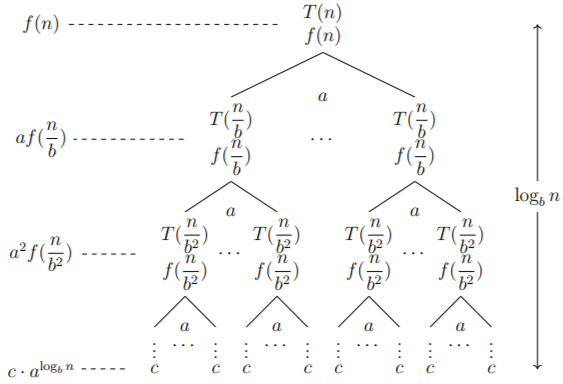
\includegraphics[width=0.7\textwidth]{image/MasterTheorem.png} \\ \\
    \end{tabular}
\end{center}

Confronta tra di loro $f(n)$ e $n^{\log_ba}$:
\begin{itemize}
    \item se vince $f(n) \Rightarrow \Theta(f(n))$
    \item se pareggiano $\Rightarrow \Theta(n^{\log_ba} \cdot \log n)$
    \item se vince $n^{\log_ba} \Rightarrow \Theta(n^{\log_ba})$
\end{itemize}

\newpage
\section{Heap Sort}

\subsection{Alberi}
\begin{itemize}
    \item binario: ogni nodo ha al massimo due figli.
    \item altezza: distanza dalla radice alla foglia più distante.
    \item ordinato: ogni nodo ha un figlio minore o uguale a se stesso.
\end{itemize}

\subsection{Alberi completi}
\begin{mdframed}
    \textbf{Albero binario completo:} ogni nodo non foglia ha due figli e ogni cammino radice-foglia ha la stessa lunghezza.
\end{mdframed}
\begin{equation*}
    \text{\# nodi} = \sum_{i=0}^k 2^i -1 \quad (h = \text{altezza})
\end{equation*}
\begin{center}
    \begin{tabular}{c}
        \\ 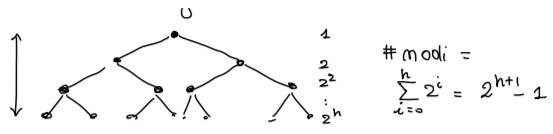
\includegraphics[width=0.6\textwidth]{image/AlberoCompleto.png} \\ \\
    \end{tabular}
\end{center}

\subsection{Alberi quasi completi}
\begin{mdframed}
    \textbf{Albero quasi completo:} ogni livello è completo, tranne eventualmente l’ultimo con foglie tutte a sx.
\end{mdframed}
\begin{center}
    \begin{tabular}{c}
        \\ 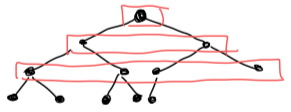
\includegraphics[width=0.3\textwidth]{image/AlberoQuasiCompleto.png} \\ \\
    \end{tabular}
\end{center}

\subsection{Heap}
\begin{mdframed}
    \textbf{Heap:} albero binario ordinato quasi completo, ma implementato come se fosse un array.
\end{mdframed}
\paragraph{Caratteristiche:}
\begin{itemize}
    \item $A[1]$ è radice
    \item Un generico nodo sta in posizione $A[i]$.
    \item Un nodo $A[2i]$ è il figlio sinistro del nodo $A[i]$
    \item Un nodo definito come nodo parent/genitore sta in posizione $A[i/2]$
    \item Lo spazio occupato effettivamente è $A.size$, la lunghezza dell'array è $A.length$.
\end{itemize}

\begin{center}
    \begin{tabular}{c}
        \\ 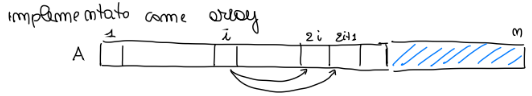
\includegraphics[width=0.6\textwidth]{image/Heap.png} \\ \\
    \end{tabular}
\end{center}

\paragraph{Max Heap}
Il Max Heap è un Heap dove:
\begin{itemize}
    \item $\forall A[i], A[i] \geq$ nodi discendenti (quindi, $A.Left[i]$,$A.Right[i]$)
    \item $\forall A[i], A[i] \leq$ nodi antenati (quindi, $A[i] \leq A.Parent[i]$)
\end{itemize}

\begin{center}
    \begin{tabular}{c}
        \\ 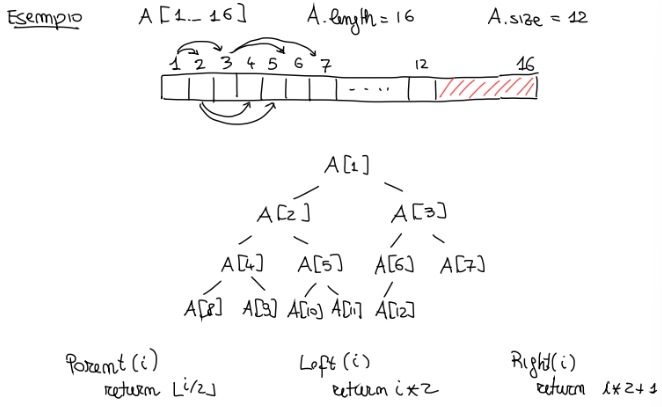
\includegraphics[width=0.7\textwidth]{image/HeapSortExample.png} \\ \\
    \end{tabular}
\end{center}

\subsection{Pseudocodice}
\begin{mdframed}
\begin{lstlisting}[language=C]
MAX-HEAPIFY(A)
1   l = LEFT(i)
2   r = RIGHT(i)
3   if l<=A.heapsize and A[l] > A[i]
4       max = l
5   else
6       max = i
7   if r<=A.heapsize and A[r] > A[max]
8       max = r
9   if max != i
10      A[i] <-> A[max]
11      MAX-HEAPIFY(A,max)
\end{lstlisting}
\end{mdframed}

\subsection{Complessità}
Dipende dall'albero, il quale avrà $n$ elementi possibili:
\begin{itemize}
    \item la complessità $O(h)$, con $h$ altezza del sottoalbero, alternativamente $O(\log(n))$.
    \begin{equation*}
        \begin{rcases}
            n \geq 2^{2^{h-1}+1} + 1 = 2^h \\
            h \leq \log_2n \\
        \end{rcases}
        \Rightarrow O(h) \;\tilde{=}\; O(\log n)
    \end{equation*}
    \item se invece fosse visto come ricorrenza, si può dimostrare con il Master Theorem
\end{itemize}




\newpage
\section{Quick Sort}
L'algoritmo di ordinamento più utilizzato e generalmente più efficiente con $O(n^2)$ come caso pessimo ed $O(n\log n)$ come caso medio e migliore è proprio quicksort.
Viene definito algoritmo "in-place", cioè un algoritmo che non ha bisogno di spazio extra e produce un output nella stessa memoria che contiene i dati.

Anche questo algoritmo è basato sul paradigma divide-et-impera, infatti, per ordinare $A[p, r]$:
\begin{itemize}
    \item Divide:
    \begin{itemize}
        \item sceglie un pivot $x$ in $A[p, r]$
        \item partiziona in $A[p, q-1] \leq x$ e $A[q+1, r] \geq x$
    \end{itemize}
    \item Impera:
    \begin{itemize}
        \item ricorre su $A[p, q-1]$ e su $A[q+1, r]$
    \end{itemize}
\end{itemize}

\subsection{Pseudocodice}
\begin{mdframed}
\begin{lstlisting}[language=C]
QUICKSORT(A,p,r)
1   q = PARTITION(A,p,r)
2   QUICKSORT(A,p,q-1)
3   QUICKSORT(A,q+1,r)
\end{lstlisting}
\end{mdframed}

\begin{mdframed}
\begin{lstlisting}[language=C]
PARTITION(A,p,r)
1   x = A[r]
2   i = p - 1
3   for j = p to r - 1
4       if A[j] <= x
5           i = i + 1
6           A[i] <-> A[j]
7   A[i + 1] <-> A[r]
8   return i + 1
\end{lstlisting}
\end{mdframed}

\subsection{Passaggi}
Per ordinare un array, seguite i passaggi seguenti:
\begin{enumerate}
    \item Si sceglie come pivot un qualsiasi valore di indice dell'array.
    \item Quindi si partiziona l'array in base al pivot.
    \item Quindi si esegue un Quicksort ricorsivo della partizione di sinistra.
    \item Successivamente, si esegue un Quicksort ricorsivo della partizione corretta.
\end{enumerate}

Diamo un'occhiata più da vicino alla partizione di questo algoritmo:
\begin{enumerate}
    \item Si sceglie un pivot qualsiasi, ad esempio il valore più alto dell'indice.
    \item Si prenderanno due variabili per puntare a sinistra e a destra dell'elenco, escludendo il pivot.
    \item La sinistra punterà all'indice più basso e la destra all'indice più alto.
    \item Ora si spostano a destra tutti gli elementi maggiori del pivot.
    \item Quindi si sposteranno tutti gli elementi più piccoli del perno nella partizione di sinistra.
\end{enumerate}

\newpage
\section{Counting Sort}
Il Counting Sort è una tecnica di ordinamento stabile, utilizzata per ordinare gli oggetti in base alle chiavi che sono piccoli numeri. Conta il numero di chiavi i cui valori sono uguali. Questa tecnica di ordinamento è efficiente quando la differenza tra le diverse chiavi non è così grande, altrimenti può aumentare la complessità dello spazio.

\subsection{Funzionamento}
\begin{enumerate}
    \item Scopri l'elemento $max$ dall'array specificato. \\
    \begin{tabular}{c}
        $max$ \\ 
    \end{tabular}
    \\
    \begin{tabular}{|c|}
        \hline
        \; 8 \; \\ 
        \hline
    \end{tabular}
    \begin{tabular}{|c|c|c|c|c|c|c|}
        \hline
        4 & 2 & 2 & 8 & 3 & 3 & 1 \\ 
        \hline
    \end{tabular}

    \item Inizializzare una matrice di lunghezza $max+1$ con tutti gli elementi $0$. Questa matrice viene utilizzata per memorizzare il conteggio degli elementi nella matrice.
    \item[]
    \begin{tabular}{|c|c|c|c|c|c|c|c|c|}
        \hline
        0 & 0 & 0 & 0 & 0 & 0 & 0 & 0 & 0 \\ 
        \hline
    \end{tabular}
    \\
    \begin{tabular}{ccccccccc}
        0 & 1 & 2 & 3 & 4 & 5 & 6 & 7 & 8 \\ 
    \end{tabular}

    \item Memorizza il conteggio di ciascun elemento nel rispettivo indice nell'array count.
    \item[]
    \begin{tabular}{|c|c|c|c|c|c|c|c|c|}
        \hline
        0 & 1 & 2 & 2 & 1 & 0 & 0 & 0 & 1 \\ 
        \hline
    \end{tabular}
    \\
    \begin{tabular}{ccccccccc}
        0 & 1 & 2 & 3 & 4 & 5 & 6 & 7 & 8 \\ 
    \end{tabular}

    \item Memorizzare la somma cumulativa degli elementi dell'array count. Aiuta a posizionare gli elementi nell'indice corretto dell'array ordinato.
    \item[]
    \begin{tabular}{|c|c|c|c|c|c|c|c|c|}
        \hline
        0 & 1 & 3 & 5 & 6 & 6 & 6 & 6 & 7 \\ 
        \hline
    \end{tabular}
    \\
    \begin{tabular}{ccccccccc}
        0 & 1 & 2 & 3 & 4 & 5 & 6 & 7 & 8 \\ 
    \end{tabular}

    \item Individuare l'indice di ogni elemento della matrice originale nell'array count. Questo dà il conteggio cumulativo.
    \item[]
    \begin{tabular}{|c|c|c|c|c|c|c|}
        \hline
        1 & 2 & 2 & 3 & 3 & 4 & 8 \\ 
        \hline
    \end{tabular}
    \\
    \begin{tabular}{ccccccc}
        0 & 1 & 2 & 3 & 4 & 5 & 6 \\ 
    \end{tabular}
    
\end{enumerate}

\subsection{Pseudocodice}
\begin{mdframed}
\begin{lstlisting}[language=C]
COUNTING-SORT(A,B,k)
1   C[0..k] = 0
2   for j = 1 to A.length
3       C[A[j]] = C[A[j]] + 1
4   for i = 1 to k
5       C[i] = C[i-1] + C[i]
6   for j = A.length to 1
7       B[C[A[j]]] = A[j]
8       C[A[j]] = C[A[j]] - 1
\end{lstlisting}
\end{mdframed}

\subsection{Complessità}
\begin{lstlisting}[mathescape=true]
C[0..k] = 0                 $\Theta(k)$
for j = 1 to A.length       $\Theta(n)$
    ...
for i = 1 to k              $\Theta(k)$
    ...
for j = A.length to 1       $\Theta(n)$
    ...
\end{lstlisting}
Somma $\Theta(n+k)$ con $k=\Theta(1) \Rightarrow \Theta(n)$

\newpage
\section{Radix Sort}
Il Radix Sort è un algoritmo di ordinamento che ordina gli elementi raggruppando prima le singole cifre tutte nella stessa attuale posizione. Quindi, ordina gli elementi in base al loro ordine crescente/decrescente. L'idea è quella di ordinare cifra per cifra con un algoritmo stabile e risolvere i problemi di memoria di Counting Sort.

\subsection{Pseudocodice}
\begin{mdframed}
\begin{lstlisting}[language=C]
Radix-SORT(A,d)
1   for j = 1 to d
2       COUNTING-SORT(A,j)
\end{lstlisting}
\end{mdframed}

\subsection{Correttezza}
\paragraph{Invariante:} $A^{j-1}$ ordinato
\paragraph{Inizializzazione:} $j=1, A^{j-1} = A^0$
\paragraph{Mantenimento:} $A^{j-1}$ ordinato e rodino rispetto a $j$

\subsection{Complessità}
\begin{itemize}
    \item $d$ volte Counting-Sort $\Theta(n+b) \Rightarrow \Theta(d(n+b)) = \Theta(n)$
    \item $d$ cifre $\Theta(1)$
    \item $b$ base $\Theta(n)$
\end{itemize}
$\begin{rcases}
    m \text{ bit} \Rightarrow m = O(\log n) \\
    r \text{ bit per cifra} \Rightarrow r = O(\log_2 n) \\
    \text{base } 2^r
\end{rcases}
\Rightarrow \Theta(\frac{m}{r}(m+2^r)) = \Theta(\frac{m}{\log n}(m+2^{\log n})) = \Theta(\frac{m}{\log n}n) = \Theta(n)$

\newpage
\section{Hash Table}
La Hash Table è una struttura di dati che memorizza i dati in modo associativo. In una tabella, i dati sono memorizzati in un formato array, dove ogni valore di dati ha un proprio valore di indice univoco. L'accesso ai dati diventa molto veloce se si conosce l'indice del dato desiderato.\\~\\
In questo modo, diventa una struttura di dati incui le operazioni di inserimento e ricerca sono molto veloci, indipendentemente dalla dimensione dei dati. La Hash Table utilizza un array come supporto di memorizzazione e usa la tecnica dell'Hash per generare un indice in cui un elemento deve essere inserito o da cui deve essere individuato. \\~\\
In particolare, si considera $U$ come insieme (universo) della chiavi, visto come $I = 0,1, \ldots,|U|-1$. La Hash Table $T$ viene vista come array $T[0,...|U|-1]$, in cui un elemento $x$ è inserito in $T[x.key]$.

\begin{center}
    \begin{tabular}{c}
        \\ 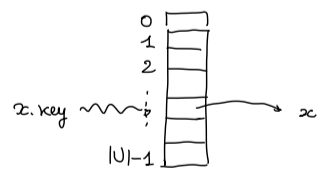
\includegraphics[width=0.4\textwidth]{image/HashTable.png} \\ \\
    \end{tabular}
\end{center}

\paragraph{Problemi:}
\begin{itemize}
    \item Non è possibile avere oggetti con la stessa chiave
    \item OK se il numero $|U|$ è piccolo
\end{itemize}

\begin{mdframed}
\begin{lstlisting}[mathescape=true]
INSERT(T,x)
1   T[x.key] = x        $\Theta(1)$
\end{lstlisting}
\end{mdframed}
\begin{mdframed}
\begin{lstlisting}[mathescape=true]
DELETE(T,x)
1   T[x.key] = NULL     $\Theta(1)$
\end{lstlisting}
\end{mdframed}
\begin{mdframed}
\begin{lstlisting}[mathescape=true]
SEARCH(k)
1   return T[k]         $\Theta(1)$
\end{lstlisting}
\end{mdframed}

\newpage
\subsection{Esempio}
\paragraph{Problema:} consideriamo che la key sia di 8 caratteri (8 bit per rappresentare un carattere). Risulta molto costosa in termini di memoria la tabella hash.
\paragraph{Obiettivo:} usare quantità di memoria proporzionale al numero di elementi da memorizzare.
\paragraph{Idea:} creazione di una tabella $T$ di dimensione $m << |U|$
\begin{equation*}
    h: U \rightarrow \{0, 1, \dots, m-1\}
\end{equation*}
Se $n>m \Rightarrow \exists\; x_1,x_2:h(x_1.key) = h(x_2.key) \Rightarrow$ conflitto \\~\\
Dove:
\begin{itemize}
    \item $n = $ \# elementi memorizzati nella tabella $T$
    \item $m = $ \# celle
\end{itemize}

La collisione verifica con $n = $ numero di elementi memorizzati se $m <<|U|$ se $n > m$. \\~\\

Il principio è il pigeonhole principle, quindi nella tabella hash, ogni valore trova una corrispondenza. 
Il pigeonhole principle è una delle idee più semplici ma più utili della matematica e può aiutarci in questo caso. 
Una versione di base dice che se ($N+1$) piccioni occupano $N$ buche, allora in qualche buca devono esserci almeno 2 piccioni. 
Quindi, se 5 piccioni occupano 4 buche, deve esserci una buca con almeno 2 piccioni.

\subsection{Chaining}
Il Chaining propone come soluzione quella di mettere sulla tabella liste dinamiche di elementi, invece che singoli elementi, in modo che in caso si incorra in una cella già occupata dopo un hashing, l'elemento venga inserito in coda (o in testa) alla lista. Nell'approccio di concatenamento, la tabella hash è una matrice di elenchi collegati, cioè ogni indice ha un proprio elenco collegato.Tutte le coppie chiave-valore mappate allo stesso indice saranno memorizzate nell'elenco collegato di quell'indice.

\begin{center}
    \begin{tabular}{c}
        \\ 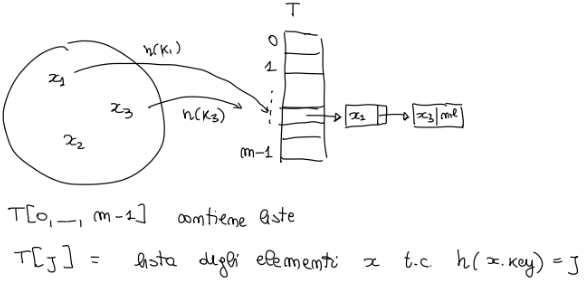
\includegraphics[width=0.7\textwidth]{image/Chaining.png} \\ \\
    \end{tabular}
\end{center}

\newpage
\begin{mdframed}
\begin{lstlisting}[mathescape=true]
INSERT(T,x)
1   T[x.key] = x           $\Theta(1)$
\end{lstlisting}
\end{mdframed}
\begin{mdframed}
\begin{lstlisting}[mathescape=true]
DELETE(T,x)
1   T[h(x.key)] = NULL     $\Theta(1)$
\end{lstlisting}
\end{mdframed}
\begin{mdframed}
\begin{lstlisting}[mathescape=true]
SEARCH(k)
1   return T[h(k)]         $\Theta(n)$
\end{lstlisting}
\end{mdframed}
L'operazione peggiore è quella di ricerca, dove alla peggio la complessità è lineare.

\section{Alberi Binari di Ricerca}
\paragraph{Albero binario:} struttura di dati ad albero composta da nodi, ognuno dei quali ha al massimo due figli, chiamati nodo destro e nodo sinistro. L'albero inizia con un singolo nodo, noto come radice. \\~\\

Matematicamente:
\begin{itemize}
    \item nodi $x$ ed elemento/valore/chiave $x.key$
    \item operazioni hanno costo $O(h)$ quando non bilanciato, $O(\log(n))$ se bilanciato
\end{itemize}

\paragraph{Definizione induttiva:}
\begin{itemize}
    \item $\varnothing$ è un albero
    \item se $r$ è un nodo, $T_1$ e $T_2$ alberi $\Rightarrow r(T_1,T_2)$ è un albero
    \item ogni nodo $x$ ha i seguenti campi:
    \begin{itemize}
        \item $x.p$
        \item $x.key$
        \item $x.left$
        \item $x.right$
    \end{itemize}
\end{itemize}

\paragraph{Operazioni possibili:}
\begin{itemize}
    \item Visita simmetrica (InOrder)
    \item Ricerca (Search)
    \item Ricerca di min e max
    \item Successore
    \item Inserimento
    \item Cancellazione
\end{itemize}

\subsection{Visita simmetrica (InOrder)}
Elencare gli elementi del sottoalbero radicato in un nodo $x$ in ordine di chiave crescente.
\begin{mdframed}
\begin{lstlisting}[language=C]
IN-ORDER(x)
1   if x != NULL
2       IN-ORDER(x.left)
3       print(x)
4       IN-ORDER(x.right)
\end{lstlisting}
\end{mdframed}
La complessità di tale operazione è lineare, dato da una visita di tutto l'albero.
\begin{equation*}
    T(n) = \begin{cases}
        c \qquad(n=0)\\
        T(k) + T(n-k-1) + d \qquad(n>0, k<n)
    \end{cases}
\end{equation*}
Stima di complessità: $T(n) = (c+d)n + c$

\newpage
\subsection{Ricerca (Search)}
Data $k$ chiave, cerca nel sottoalbero radicato nel nodo $x$ un nodo con chiave $k$.
\begin{mdframed}
\begin{lstlisting}[language=C]
SEARCH(x,k)
1   if (x == NULL) or (x.key == k)
2       return x
3   else if (k < x.key)
4       return SEARCH(x.left,k)
5   else
6       return SEARCH(x.right,k)
\end{lstlisting}
\end{mdframed}
La complessità, nel caso peggiore, è la ricerca che continua fino ad una foglia ed il cammino radice-foglia è quello massimo. Complessità: $O(h)$.
\begin{mdframed}
\begin{lstlisting}[language=C]
SEARCH(x,k)
1   while (x != NULL) and (x.key != k)
2       if (k < x.key)
3           x = x.left
4       else
5           x = x.right
6   return x
\end{lstlisting}
\end{mdframed}
Se dobbiamo esaminare tutto l'albero, nel caso peggiore avremo una complessità $\Theta(n)$ sulla base di una relazione di ricorrenza $T(n) = c + T(k) + T(n-k-1)$. 

\subsection{Ricerca di min e max}
Ricerca continuando ad andare verso sx oppure continuando ad andare verso dx. Per entrambi, la complessità è data dall'altezza dell'albero, in generale $O(h)$.
\begin{multicols}{2}
\begin{mdframed}
\begin{lstlisting}[language=C]
MIN(T)
1   x = T.root
2   if x == NULL
3       return NULL
4   else
5       while x.left != NULL
6           x = x.left
7       return x
\end{lstlisting}
\end{mdframed}
\begin{mdframed}
\begin{lstlisting}[language=C]
MAX(T)
1   x = T.root
2   if x == NULL
3       return NULL
4   else
5       while x.right != NULL
6           x = x.right
7       return x
\end{lstlisting}
\end{mdframed}
\end{multicols}

\subsection{Successore}
Si intende il nodo elencato dopo un nodo $x$ passato come parametro in una visita simmetrica. \\~\\
Dato $x \in ABR$:
\begin{itemize}
    \item minimo tra i nodi più grandi di $x$
    \item nodo che segue $x$ in una visita \verb|InOrder|
    \item se $x$ ha sottoalbero dx non vuoto $\Rightarrow$ il successore è $\min(x.right)$
    \item se $x$ non ha sottoalbero dx $\Rightarrow$ il successore è ilpiù vicino antenato di $x$ è nel sottoalbero sx
\end{itemize}
\begin{mdframed}
\begin{lstlisting}[language=C]
SUCCESSOR(x)
1   if x.right != NULL
2       return MIN(x.right)
3   else
4       y = x.p
5       while (y != NULL) and (x == y.right)
6           x = y
7           y = y.p
8       return y
\end{lstlisting}
\end{mdframed}
Complessità: $O(h)$.

\subsection{Inserimento}
La funzione \verb|Insert| viene utilizzata per aggiungere un nuovo elemento in un albero di ricerca binario in una posizione appropriata. \\~\\
La funzione \verb|Insert| deve essere progettata in modo tale da non violare la proprietà dell'albero di ricerca binario a ogni valore.
\begin{enumerate}
    \item Allocare la memoria per l'albero.
    \item Impostare la parte dei dati sul valore e impostare il puntatore sx e dx dell'albero su NULL.
    \item Se l'elemento da inserire sarà il primo elemento dell'albero, i puntatori sx e dx di questo nodo punteranno a NULL.
    \item In caso contrario, controlla se l'elemento è inferiore all'elemento radice dell'albero. 
    \item Se è vero, esegue ricorsivamente l'operazione con la sx della radice.
    \item Se è falso, allora si esegue questa operazione ricorsivamente con il sottoalbero dx della radice.
\end{enumerate}
\begin{mdframed}
\begin{lstlisting}[language=C]
INSERT(T,z)
1   x = T.root
2   y = NULL
3   while x != NULL
4       y = x
5       if z.key < x.key
6           x = x.left
7       else
8           x = x.right
9   z.p = y
10  if y == NULL
11      T.root = z
12  else
13      if z.key < y.key
14          y.left = z
15      else
16          y.right = z
\end{lstlisting}
\end{mdframed}
Complessità: $O(h)$.

\section{RedBlack Tree}
I RB-Tree sono ABR i cui nodi hanno un bit extra riservato ad un campo colore $x.color$, che può essere: $red$ per il rosso, $black$ per il nero. \\~\\
Un RB-Tree soddisfa le seguenti proprietà:
\begin{itemize}
    \item Proprietà RB: ogni nodo è colorato, rosso o nero
    \item Proprietà della radice: la radice è nera
    \item Proprietà delle foglie: ogni foglia (NULL) è nera
    \item Proprietà del rosso: se un nodo rosso ha dei figli, questi sono sempre neri
    \item Proprietà Depth: per ogni nodo, qualsiasi percorso semplice da questo nodo a qualsiasi foglia discendente ha la stessa profondità nera (il numero di nodi neri)
\end{itemize}
\begin{center}
    \begin{tabular}{c}
        \\ 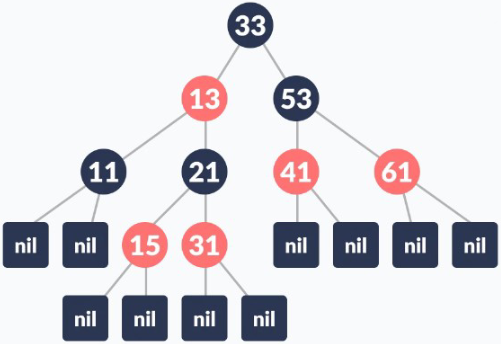
\includegraphics[width=0.7\textwidth]{image/RB-Tree.png} \\ \\
    \end{tabular}
\end{center}
Le operazioni degli RB-Tree saranno chiaramente simili a prima, in particolare:
\begin{itemize}
    \item \verb|Search|
    \item \verb|Max|
    \item \verb|Min|
    \item \verb|Successor|
    \item \verb|Precessor| (se $x$ ha 2 figli, il suo predecessore è il valore max nel suo sottoalbero sx e il suo successore il valore min nel suo sottoalbero dx. Se non ha un figlio a sx, il predecessore di un nodo è il suo primo antenato a sx)
    \item \verb|Insert| (difficile mantenere la colorazione)
    \item \verb|Delete| (difficile mantenere la colorazione)
\end{itemize}
La complessità delle operazioni è sempre data dall'altezza $h$ dell'albero, come $h = O(\log(n))$ con $h \leq 2 \log_2 (n+1)$. \\~\\

\subsection{Rotation}
Nell'operazione di \verb|Rotation|, le posizioni dei nodi di un sottoalbero vengono scambiate. \\
Esistono 2 tipi di rotazioni:
\begin{itemize}
    \item Rotazione a sx: la disposizione dei nodi a dx viene trasformata in quella dei nodi a sx
\begin{mdframed}
\begin{lstlisting}[language=C]
Left(T,x)
1   y = x.right
2   x.right = y.left
3   x.right.p = x
4   Transplant(T,x,y)
5   y.left = x
6   x.p = y
\end{lstlisting}
\end{mdframed}
    \item Rotazione a dx: la disposizione dei nodi a sx viene trasformata in quella del nodo a dx
\begin{mdframed}
\begin{lstlisting}[language=C]
Right(T,y)
1   x = y.left
2   y.left = x.right
3   if x.right != T.NULL
4       x.right.p = y
5   x.p = y.p
6   if y.p == T.NULL
7       T.root = x
8   else if y == y.p.right
9       y.p.right = x
10  else y.p.left = x
11      x.right = y
12      y.p = x
\end{lstlisting}
\end{mdframed}
\end{itemize}

\subsection{Inserimento}
Vogliamo inserire $z$ nell'albero $T$. L'idea è quella di porre $z$.$color = RED$(migliore, in quanto andando a modificare il numero di nodi neri, cambia l'altezza nera, e la cosa è difficile da sistemare).
\begin{itemize}
    \item Se violo la proprietà 2 (radice deve essere nera) $\Rightarrow z.color = BLACK$
    \item Se violo la proprietà 4 (se un nodo rosso ha dei figli, questi sono sempre neri) $\Rightarrow$ risolvo localmente e sposto verso l'alto il problema
\end{itemize}
\begin{mdframed}
\begin{lstlisting}[language=C]
RB-INSERT(T,z)
1   INSERT(T,z)
2   z.color = RED
3   RB-INSERT-FIXUP(T,z)
\end{lstlisting}
\end{mdframed}

Abbiamo dei problemi rispetto alle proprietà degli RB:
\begin{itemize}
    \item $z.color = RED$
    \item $z.p.color = RED$
\end{itemize}
Analizziamo il macrocaso $z.p$ è figlio sinistro. Abbiamo due possibilità per y:
\begin{itemize}
    \item $y.color = RED$ \\~\\ Inverto il colore di $z.p.p$ con quello dei figli $\Rightarrow$ risolviamo localmente rimandiamo il problema verso l'alto
    \item $y.color = BLACK$ \\~\\ Possiamo distinguere due sottocasi:
    \begin{itemize}
        \item $z$ figlio dx $\Rightarrow$ applico \verb|Left|$(T,z.p)$
        \item $z$ figlio sx $\Rightarrow$ scambio i colori di $z.p.p$ con $z.p \Rightarrow$ applico \verb|Right|$(T,z.p.p)$
    \end{itemize}
\end{itemize}
\begin{mdframed}
\begin{lstlisting}[language=C]
RB-INSERT-FIXUP(T,z)
1   while z.p.color == RED
2       if z.p == z.p.p.left
3           y = z.p.p.right
4           if y.color == RED
5               z.p.p.color = RED
6               z.p.color = BLACK
7               y.color = BLACK
8               z = z.p.p
9           else
10               if z == z.p.right
11                   LEFT(T,z,p)
12                   z = z.left
13               z.p.color = BLACK
14               z.p.p.color = RED
15               RIGHT(T,z.p.p)
16       else
17          ...
18   T.root.color = BLACK
\end{lstlisting}
\end{mdframed}
Complessità $O(\log n) + \max 2$ rotazioni \\~\\

Quale proprietà RB può essere violata quando si chiama \verb|RB-INSERT-FIXUP|
\begin{itemize}
    \item Proprietà 1: continua a valere
    \item Proprietà 2: violata quando $z$ è la radice e $z$ è rosso
    \item Proprietà 3: continua a valere
    \item Proprietà 4: violata quando sia $z$ che $p[z]$ sono rossi
    \item Proprietà 5: continua a valere, perché coloriamo $z$ di rosso
\end{itemize}

I 3 casi seguenti violeranno le proprietà dell'albero rosso-nero e i passaggi successivi mostrano come \verb|RB-INSERT-FIXUP| funziona per ricorrere alle proprietà rosso-nere:
\begin{itemize}
    \item caso 1: lo zio $y$ di $z$ è rosso
    \begin{enumerate}
        \item colorare $p[z]$ e $y$ di nero
        \item colorare $p[p[z]]$ di rosso
        \item spostate il puntatore $z$ di due livelli su $p[p[z]]$
    \end{enumerate}
    \item caso 2: lo zio di $z$, $y$, è nero e $z$ è un figlio dx
    \begin{enumerate}
        \item eseguire la rotazione a sx su $z$
        \item passare al caso 3
    \end{enumerate}
    \item caso 3: lo zio di $z$, $y$, è nero e $z$ è un figlio di sx
    \begin{enumerate}
        \item colorare $p[z]$ di nero
        \item colorare $p[p[z]]$ di rosso
        \item eseguite la rotazione a dx su $p[p[z]]$
    \end{enumerate}
\end{itemize}

\subsection{Cancellazione}
Per la cancellazione \verb|RB-Delete|$(T,z)$ distinguiamo 2 casi:
\begin{itemize}
    \item $z$ ha un figlio
    \item $z$ ha due figli
\end{itemize}
Ci comportiamo allo stesso modo della \verb|Delete|$(T,z)$ per un ABR, facendo però un ulteriore accorgimento:
\begin{itemize}
    \item se $z.color = RED \Rightarrow$ non ho problemi
    \item se $z.color = BLACK \Rightarrow$ risolvo localmenteo e sposto verso l'alto il problema
\end{itemize}
Dunque, in seguito alla \verb|Delete|$(T,z)$, il nodo $x$ che ha preso il posto di $z$ ne "assorbirà" il colore diventando doppiamente $BLACK$. Abbiamo due casi:
\begin{itemize}
    \item $x$ è figlio sx (noi analizziamo solo questo, immagine)
    \item $x$ è figlio dx
\end{itemize}
Abbiamo due possibilità per $w$:
\begin{itemize}
    \item $w.color = RED$
    \begin{enumerate}
        \item scambio i colori di $w$ con $x.p$
        \item applico \verb|Left|$(T,x,p)$ 
    \end{enumerate}
    \item $w.color = BLACK$ \\~\\
    Possiamo distinguere 3 sottocasi:
    \begin{itemize}
        \item $w.left.color = BLACK$ e $w.right.color = BLACK$
        \begin{enumerate}
            \item $x$ cede un suo $BLACK$ a $x.p$ e $w$ diventa per forza $RED$
            \item risolviamo localmente e rimandiamo il problema in alto
        \end{enumerate}
        \item $w.right.color = BLACK$
        \begin{enumerate}
            \item scambio i colori di $w$ con $w.left$
            \item applico \verb|Right|$(T,w)$
        \end{enumerate}
        \item $w.right.color = RED$
        \begin{enumerate}
            \item scambio i colori di $x.p$ con $w$ e $w.right$ diventa $BLACK$
            \item applico \verb|Left|$(T,x,p)$
        \end{enumerate}
    \end{itemize}
\end{itemize}
Complessità $O(\log n) + \max 3$ rotazioni

\newpage
\begin{mdframed}
\begin{lstlisting}[language=C]
RB-DELETE(T,z)
1   if z.left == T.NULL && z.right == T.NULL
2       then y = z
3       else y = TREE-SUCCESSOR(z)
4   if y.left != T.NULL
5       then x = y.left
6       else x = y.right
7   x.p = y.p
8   if y.p == T.NULL
9       then T.root = x
10      else if y == y.p.left
11          then y.p.left = x
12          else y.p.right = x
13  if y != z
14      then z.key = y.key
15  if y.color == BLACK
16      then RB-DELETE-FIXUP(T,x)
17  return y
\end{lstlisting}
\end{mdframed}
\begin{mdframed}
\begin{lstlisting}[language=C]
RB-DELETE-FIXUP(T,x)
1   while x != T.root && x.color == BLACK
2       if x == x.p.left
3           then w = x.p.right
4               if w.color == RED
5                   then w.color = BLACK
6                       x.p.color = RED
7                       Left(T,x.p)
8               if w.left.color == BLACK && w.right.color == BLACK
9                   then w.color = RED
10                      x = x.p
11                  else if w.right.color == BLACK
12                      then w.left.color = BLACK
13                          w.color = RED
14                          Right(T,w)
15                          w = x.p.right    
16                  w.color = x.p.color
17                  x.p.color = BLACK
18                  w.right.color = BLACK
19                  Left(T,x.p)
20                  x = T.root
21          else (same with Left and Right inverted)
22  x.color = BLACK
\end{lstlisting}
\end{mdframed}

\newpage

\section{Divide et Impera}
Il metodo Divide et Impera, non ha memoria, ogni volta che si calcola una soluzione, il processo richiede di ricalcolare la sottoistanza del problema che lo ha risolto, generando quindi un problema di sottoistanze ripetute. \\~\\

Il Divide et Impera, possiede 2 fasi:
\begin{itemize}
    \item \textbf{Top-down:} con cui vengono generate le istanze risolte divide il problema originale in un numero di sottoproblema (divide), risolvendo i problemi ricorsivamente (impera) e combinando le soluzioni dei sottoproblemi nella soluzione ai sottoproblemi originali (combine)
    \item \textbf{Bottom-up:} normalmente non ricorsiva ma iterativa
    \begin{itemize}
        \item caratterizza la struttura delle soluzioni ottimali
        \item definiscono ricorsivamente i valori delle soluzioni ottimali
        \item calcola il valore delle soluzioni ottimali
        \item costruisce una soluzione ottimale a partire dalle informazioni calcolate
    \end{itemize}
    Sinteticamente, si elaborano le soluzioni alle istanze presenti.
\end{itemize}
\begin{center}
    \begin{tabular}{c}
        \\ 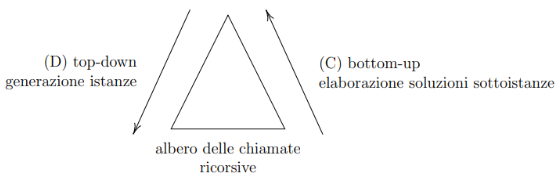
\includegraphics[width=0.8\textwidth]{image/T-D_B-U.png} \\ \\
    \end{tabular}
\end{center}
L'approccio della programmazione dinamica salta completamente l'approccio top-down, normalmente usando algoritmi iterativi per evitare di dover calcolare la soluzione. La programmazione Divide et Impera usa entrambi gli approcci e normalmente in modo ricorsivo.

\subsection{Memoizzazione}
È possibile mantenere i vantaggi del Top-down e quindi anche del Divide et Impera senza incorrere nel problema del ricalcolo delle soluzioni, usando il concetto di memoizzazione. \\~\\

Un algoritmo memoizzato è costituito da 2 subroutine/procedure:
\begin{itemize}
    \item \textbf{routine di inizializzazione:}
    \begin{itemize}
        \item risolve direttamente i casi base
        \item inizializza una struttura dati "tabella" che contiene le soluzioni ai casi base ed elementi per tutte le sottoistanze da calcolare inizializzate ad un valore di default
        \item invoca la struttura ricorsiva
    \end{itemize}
    \item \textbf{routine ricorsiva:}
    \begin{itemize}
        \item segue il codice del Divide et Impera preceduto da un test sulla tabella per verificare se la soluzione è già stata calcolata e memorizzata
        \item se si, ritorna
        \item altrimenti si calcola ricorsivamente e si memorizza nella struttura
    \end{itemize}
\end{itemize}

\subsection{Ottimizzazione}
Ora, consideriamo i problemi di ottimizzazione, per cui si cerca di trovare una cosiddetta soluzione ottima, definita come $s*$, definendo tutto come segue:
\begin{itemize}
    \item $I =$ insieme delle istanze
    \item $S =$ insieme delle soluzioni
    \item $\forall i \in I, S(i) = \{s \in S: (i,s) \in \Pi\} =$ insieme delle soluzioni ammissibili
    \item $c: S \rightarrow \mathbb{R} =$ funzione di costo
    \item $i \in I, s* \in S(i): c(s*) = \min / \max \{c(s): s \in S(i)\}$
\end{itemize}

Paradigma generale sullo sviluppo di un algoritmo di programmazione dinamica. Caratteristiche dei problemi:
\begin{itemize}
    \item struttura ricorsiva: la soluzione ottima si ottiene come funzione di soluzioni ottime di sottoistanze ("proprietà di sottostruttura ottima", quindi il fatto che ogni soluzione contenga già soluzioni precedenti)
    \item esistenza di sottoistanze ripetute ("overlapping subproblems"), teoricamente risolvibili in maniera ottima (altrimenti, conviene applicare Divide et Impera)
    \item spazio dei sottoproblemi piccolo: poche sottoistanze che possono contribuire a crearela soluzione al livello superiore
\end{itemize}

Ricetta:
\begin{itemize}
    \item caratterizza la struttura di una soluzione ottima $s*$ in funzione di soluzioni ottime $s_1*, \ldots, s_k*$ di sottoistanze di taglia inferiore
    \item determinare una relazione di ricorrenza del tipo $c(s*) = f(c(s_1*), \ldots, c(s_k*))$
    \item calcola $C(S*)$ utilizzando la ricorrenza ma impostando il calcolo in maniera bottom-up (iterativo) oppure memoizzando il codice Divide et Impera basato sulla definizione di $C(S*)$
    \item (opzionale) mantieni informazioni strutturali aggiuntive che permettono di ricostruire $S*$
\end{itemize}
\section{Longest Common Subsequence}
Longest Common Subsequence (LCS) e' un problema di ottimizzazione, ovvero si cerca di trovare una soluzione ottima.
\subsection{Problema di Ottimizzazione}
\begin{mdframed}
    Date 2 stringhe $X,Y$ determina $Z$ tale che:
    \begin{itemize}
        \item $Z$ è sottosequenza di $X$ e $Y$
        \item $Z$ è la più lunga tra tutte le sottosequenze comuni
    \end{itemize}
\end{mdframed}
Avendo complessità esponenziale, si cerca di individuare una struttura ricorsiva, cioè una proprietà di sottostruttura. La LCS deve "nascondere" al suo interno LCS di qualche stringa più piccola di $X$ e $Y$.
\begin{equation*}
\begin{rcases}
    X = \langle X',a \rangle \\
    Y = \langle Y',b \rangle
\end{rcases} \Rightarrow Z \text{ è la stringa più lunga tra } \verb|LCS|(X',Y) \text{ e } \verb|LCS|(X,Y')
\end{equation*}
Spazio sottoproblemi: $S = \{ \verb|LCS|(X_i,Y_j): 0 \leq i \leq m, 0 \leq j \leq n \} \Rightarrow |S| = (m+1)(n+1)$

\subsection{Proprietà di Sottostruttura}
Ottima per il sottoproblema \verb|LCS|$(X_i,Y_j)$
Dati:
\begin{itemize}
    \item $X_i = \langle x_1,x_2,\dots,x_i \rangle$
    \item $Y_i = \langle y_1,y_2,\dots,y_j \rangle$
\end{itemize}
Sia $Z = \langle z_1,z_2,\dots,z_k \rangle = \verb|LCS|(X_i,Y_j)$
\begin{itemize}
    \item caso base: $i = j = 0 \Rightarrow Z = \varepsilon$
    \item $i,k>0$: se $x_i = y_i$ \\
    $\Rightarrow z_k = x_i(= y_i)$ \\
    $\Rightarrow Z_{k-1} = \verb|LCS|(X_{i-1},Y_{j-1})$
    \item $i,j>0$: se $x_i \not= y_j$ \\
    $\Rightarrow Z$ è la stringa di lunghezza max tra \verb|LCS|$(X_{i-1},Y_j)$ e \verb|LCS|$(X_i,Y_{j-1})$
\end{itemize}

\subsection{Ricorrenza sui Costi}
La scrittura della ricorrenza sui costi è il secondo passo per costruire un algoritmo di programmazione dinamica.
\begin{equation*}
l(i,j) = |\verb|LCS|(X_i,Y_j)| = 
\begin{cases}
    \text{caso base: se } i=0, j=0 \qquad\;\; 0 \\
    \text{caso 1: se } i,j>0, x_i = x_j \qquad\; l(i-1,j-1)+1 \\
    \text{caso 2: se } i,j>0, x_i \not= x_j \qquad \max(l(i,j-1),l(i-1,j))
\end{cases}
\end{equation*}
Ci interessa calcolare $l(m,n)$

\subsection{Modello di Costo: confronto tra caratteri}
\begin{equation*}
    T(n,m) =
    \begin{cases}
        \text{se } n,m=0 \qquad 0 \\
        \text{se } n,m>0 \qquad T(n-1,m) + T(n,m-1) + 1 \\
    \end{cases}
\end{equation*}

\section{Longest Increasing Subsequence}
\begin{mdframed}
    \textbf{Def} \quad Dato un alfabeto $\sum$ totalmente ordinato ($\forall\; a,b \in \sum \quad a<b, a=b, a>b$) e dato $X = \langle x_1,x_2,\ldots,x_n \rangle$, si dice che $Z = \langle z_1,z_2,\ldots,z_k \rangle$ è sottosequenza crescente di $X (Z = IS(X))$
\end{mdframed}

\subsection{Problema di Ottimizzazione}
Determinare la più lunga sottosequenza crescente di $X(Z = LIS(X))$
\begin{mdframed}
    \textbf{Def} \quad $Z = \overline{LIS}(X_i)$ è la più lunga tra le $IS(X_i)$ con $Z = \langle z_1,z_2,\ldots,z_k \rangle = \langle x_{i_1},x_{i_2},\ldots,x_{i_k} \rangle$ con $i_k = i$
\end{mdframed}
Casi:
\begin{itemize}
    \item \textbf{fortunato:} $Z_k < X_{i+1} \Rightarrow LIS(X_{i_1}) = \langle Z^i, X_{i+1} \rangle$
    \item \textbf{sfortunato:} $Z_k \geq X_{i+1} \Rightarrow LIS(X_{i_1}) = \langle Z^i \rangle \Rightarrow$ NO perché $X_{i+1}$ è una $LIS(X^i) \Rightarrow |LIS(X_{i+1})| = |LIS(X_i)| + 1$
\end{itemize}

\subsection{Proprietà di Sottostruttura Ottima}
\begin{itemize}
    \item caso base: $\overline{LIS}(X_1) = \langle x_1 \rangle (= LIS(X_1))$
    \item caso $i>1$
    \begin{itemize}
        \item $\forall\; j : 1 \leq j \leq i, \quad x_j \geq x_i$ \\
              $\overline{LIS}(X_i) = \langle x_i \rangle (= LIS(X_i))$
        \item $\exists\; \overline{j} : 1 \leq n \overline{j} \leq i, \quad x_{\overline{j}} < x_i$ \\
              $|\overline{LIS}(X_i)| \geq 2$ \\
              $\overline{LIS}(X_i) = \langle z_1,z_2, \ldots, z_k \rangle = \langle Z_{k-1}, x_i \rangle$ con $Z_{k-1} : |Z_{k-1}| = \max_{1 \leq j \leq i} \{\overline{LIS}(X_j) : x_j < x_i\}$
    \end{itemize}
\end{itemize}

\subsection{Ricorrenza sui Costi}
Definisco;
\begin{itemize}
    \item $l(i) = |\overline{LIS}(X_i)|$
    \item $l(i) = \begin{cases}
        \text{se } i=1 \qquad 1 \\
        \text{se } i>1 \qquad 1 + \max_{1 \leq j < i}\{l(j): x_j < x_i\}
    \end{cases}$
\end{itemize}
Per costruire la sottosequenza:
\begin{equation*}
    \overline{LIS}(X_i) = 
    \begin{cases}
        \langle x_i \rangle \\
        \langle \overline{LIS}(X_{\overline{j}}),x_i \rangle \qquad (1 \leq \overline{j} < i)
    \end{cases}
\end{equation*}
Informazioni addizionali:
\begin{itemize}
    \item $prev(i) = \begin{cases}
        0 \\
        \overline{j}
    \end{cases}$
    \item $len = \max _{1 \leq i \leq n} \{l(i)\}$
    \item $end = i \qquad \overline{LIS}(X_i) = LIS(X)$
\end{itemize}

\newpage
La LIS è quindi composta da $\langle \dots, X_(prev(prev(i))), X_(prev), X_i \rangle$ \\
Non possiamo usare un algoritmo ricorsivo, in quanto abbiamo diversi sottoproblemi ripetuti.
Scriviamo quindi l'algoritmo bottom-up, a partire da $\overline{LIS}(X_1)$.
\begin{mdframed}
\begin{lstlisting}[language=C]
LIS(x)
1   L[1] = 1
2   len = 1
3   end = 1
4   prev[1] = 0
5   for i = 2 to n
6       L[i] = 1
7       prev[i] = 0
8       for j =1 to i-1
9           if x_j < x_i
10              if L[i] < 1 + L[j]
11                  L[i] = 1 + L[j]
12                  prev[i] = j
13      if len < L[i]
14          len = L[i]
15          end = i
16  return (len, prev, end)
\end{lstlisting}
\end{mdframed}
\begin{itemize}
    \item inizializzo tutti i valori di ricerca della sottosequenza
    \item nel primo ciclo, inizializzo la lunghezza dell'elemento attuale e inizializzo l'elemento precedente
    \item nel secondo ciclo, che parte dalla fine per poter ottimizzare il proprio calcolo e avere già la soluzione ottimale partendo dal primo elemento, confronto l'elemento i-esimo con l'elemento j-esimo
    \item se fosse minore, si salva l'elemento attuale j-esimo nell'array i-esimo e si salva la lunghezza raggiunta e dove si ferma
\end{itemize}
\begin{mdframed}
\begin{lstlisting}[language=C]
R-PRINT(X,prev,i)
1   if prev[i] != 0
2       R-PRINT(X,prev,prev[i])
3   print(x_i)
\end{lstlisting}
\end{mdframed}
\paragraph{Complessità} $\sum_{i=2}^n \sum_{j=1}^{i\;1}1 = \sum_{i=2}^n (i-1) = \frac{n(n-1)}{2} = \Theta(n^2)$ \\~\\
La pratica è questa:
\begin{itemize}
    \item considero il mio array delle sottostringhe e cerco di trovare le sottosequenze che crescono
    \item nell’array delle lunghezze, consideriamo che noi teniamo traccia delle sottosequenze attuali che si incrementano, considerano che teniamo solo le sottosequenze che, a parità di numero di elementi, hanno un valore nella stessa posizione minore. Non avremo mai due sottosequenze che si incrementano con lo stesso numero di elementi
    \item noi confrontiamo gli elementi della sottostringa uno per uno; l'array delle lunghezze si aggiorna "per riga", quindi, salviamo solo le posizioni in cui la lunghezza della sottostringa sottostante aumenta, tale da poter individuare facilmente qual è la sottosequenza migliore
\end{itemize}

\newpage
\section{Shortest Palindrome Completion}
\begin{mdframed}
    \textbf{Def} \quad Una stringa $Z = \langle z_1,z_2,\ldots,z_n \rangle$ è palindroma se $z_{1+h} = z_{m-h} \quad (\forall\; 0 \leq h \leq m-1)$
\end{mdframed}
\paragraph{Problema:} Data $X = \langle x_1,x_2,\ldots,x_n \rangle$ un complemento palindromo di $X$ è una stringa $Z = CP(X) = \langle z_1,z_2,\ldots,z_m \rangle$ con $m \geq n$ tale che:
\begin{itemize}
    \item $Z$ e' palindroma
    \item $X$ è sottosequenza di $Z$
\end{itemize}
\subsection{Proprietà di Sottostruttura Ottima}
Casi:
\begin{itemize}
    \item $i=j$ \\~\\
          $X = \langle x_i \rangle$ \\
          $CP(X_{i \ldots j}) = X_{i \ldots j}$ \\
          $|CP(X_{i \ldots j})| = |X_{i \ldots j}|$
    \item $j = i+1$ \\~\\
          $X_{i \ldots j} = \langle x_i,x_{i+1} \rangle$
    \item $X_{i \ldots j} = \langle x_i,x_{i+1},\ldots,x_j \rangle$
    \begin{itemize}
        \item $x_i = x_j$ \\~\\
              $Z = CP(X_{i \ldots j})$ \\
              $z_1 = z_k = x_i (= x_j)$ \\
              $Z_{2 \ldots k-1} = CP(X_{i+1 \ldots j-1})$
        \item $x_i \not= x_j$
        \begin{itemize}
            \item $z_1 = z_k = x_i$ \\
                  $Z_{2 \ldots k-1} = CP(X_{i+1 \ldots j})$
            \item $z_1 = z_k = x_j$ \\
                  $Z_{2 \ldots k-1} = CP(X_{i \ldots j-1})$
        \end{itemize}
    \end{itemize}
\end{itemize}

\subsection{Ricorrenza sulle Lunghezze}
Definisco:
\begin{itemize}
    \item $l(i,j) = |CP(X_{i \ldots j})|$
    \item $l(i,j) = \begin{cases}
        \text{se } i = j \qquad\qquad\qquad\;\;\;\;\; 1 \\
        \text{se } j = i+1, x_i = x_j \qquad 2\\
        \text{se } j = i+1, x_i \not= x_j \qquad 3\\
        \text{se } j > i+1, x_i = x_j \qquad 2 + l(i+1,j-1)\\
        \text{se } j > i+1, x_i \not= x_j \qquad 2 + \min\{l(i+1,j),l(i,j-1)\}
    \end{cases}$
\end{itemize}

\newpage
\subsection{Pseudocodice}
\begin{mdframed}
\begin{lstlisting}[language=C]
SPC(X)
1   n = X.length
2   for i=1 to n-1
3       L[i,j] = 1
4       if x_i = x_{i+1}
5           L[i,i+1] = 2
6       else
7           L[i,i+1] = 3
8   L[n,n] = 1
9   for l=3 to n
10      for i=1 to n-l+1
11          j = i+l-1
12          if x_i = x_j
13              L[i,j] = 2 + L[i+1,j-1]
14          else
15              L[i,j] = 2 + min(L[i+1,j],L[i,j-1])
16  return L[1,n]
\end{lstlisting}
\end{mdframed}
Per l’algoritmo:
\begin{itemize}
    \item salvo la lunghezza iniziale della parola
    \item inizializzo l'array delle lunghezze e copro i casi base (stringhe con 2 caratteri uguali a stringhe consecutive (metto 2) o stringhe con 2 caratteri uguali non consecutive (metto 3))
    \item procedo con una scansione diagonale (con $l$ che parte da 3 avendo esaminato i casi base palindromo e assicurandomi di non avere stringa palindroma di 1-2 caratteri)
    \item l'altro ciclo esclude tutte le stringhe già controllate (lunghezza 1/2)
    \item se le stringhe sono uguali, continuo a cercare in diagonale
    \item altrimenti, scelgo la stringa di lunghezza minima (perché cerco di ottimizzare il problema e quindi scelgo la stringa più corta da controllare) a sinistra e sotto
\end{itemize}
\paragraph{Complessità} $\Theta(n^2)$
\begin{equation*}
    \sum_{i=1}^{n-1} + \sum_{l=3}^{n} \sum_{i=1}^{n-l+1} =
    \sum_{i=1}^{n-1} + \sum_{l=3}^{n}(n-l+1) =
    \sum_{i=1}^{n-1} + \sum_{i=2}^{n-1}(n-i) =
    \sum_{i=1}^{n-1}(n-i) =
    \sum_{j=1}^{n-1}j =
    \frac{n(n-1)}{2} =
    \Theta(n^2)
\end{equation*}

\newpage
\section{Algoritmi Greedy}
Un algoritmo Greedy è un approccio per risolvere un problema selezionando la migliore opzione disponibile al momento. Non si preoccupa di sapere se il risultato migliore attuale porterà al risultato ottimale complessivo. L'algoritmo non inverte mai la decisione precedente, anche se la scelta è sbagliata. Funziona con un approccio Top-Down. \\~\\
In particolare:
\begin{itemize}
    \item sono semplici, costruiscono l’ottimo per scelte successive
    \item possiedono la proprietà di sottostruttura ottima per la decisione che prendono
    \item risolvono un solo sottoproblema
    \item hanno un campo di applicazione limitato
\end{itemize}

\subsection{Problema di Ottimizzazione}
Determinare un sottoinsieme di massima cardinalità di attività mutuamente compatibili (cioè compatibili a coppie).

\subsection{Proprietà di Sottostruttura Ottima}
Sia $A_{ij}^*$ un sottoinsieme di attività compatibili di $S_{ij}$ di cardinalità massima
\begin{itemize}
    \item caso base: $S_{ij} = \varnothing \Rightarrow A_{ij}^* = \varnothing$
    \item caso generale: $S_{ij} \not= \varnothing$
    \begin{itemize}
        \item $A_{ij}^* = \varnothing$
        \item se $a_k \in A_{ij}^*$ allora $A_{ij}^* = A_{ik}^* \cup A_{kj}^*$ dove $A_{ik}^*$ e $A_{kj}^*$ sono soluzioni ottime per $S_{ik}$ e $S_{kj}$
    \end{itemize}  
\end{itemize}

\subsection{Ricorrenza dei Costi}
Definisco:
\begin{itemize}
    \item $c(i,j) = |A_{ij}^*|$
    \item $c(i,j) = \begin{cases}
        S_{ij} = \varnothing \qquad 0 \\
        S_{ij} \not= \varnothing \qquad 1 + \max_{a_k \in S_{ij}} \{c(i,k) + c(k,j)\}
    \end{cases}$
\end{itemize}
\paragraph{Complessità} $\Theta(n^3)$

\subsection{Aspetto Greedy}
Aspetto greedy del problema: $\exists$ attività di $S_{ij}$ che sta sicuramente in $A_{ij}^*$.
Qual è questa attività? \\~\\
Sia $a_m$ l'attività tale che
\begin{equation*}
    f_m = \min\{f_k: a_k \in S_{ij}\}
\end{equation*}
Se $S_{ij} \not= \varnothing$ allora
\begin{itemize}
    \item $\exists A_{ij}^*$ soluzione ottima, tale che $a_m \in A_{ij}^*$
    \item il sottoproblema $S_{im} = \varnothing$
\end{itemize}
\paragraph{Strategia}
\begin{itemize}
    \item scegliere $a_m$
    \item risolvere $S_{mj}$ \quad (perché $A_{ij}^* = \{a_m\} \cup A_{mj}^*$)
\end{itemize}
Per risolvere $S = S_{(0 \; n+1)}$ viene invocata la soluzione solo di problemi del tipo $S_{(m \; n + 1)}$ spazio dei sottoproblemi è ridotto da quadratico a lineare: al più $n+1$ sottoproblemi, cioè quelli che vanno da $m=0$ ad $m = n+1$.
\begin{mdframed}
\begin{lstlisting}[mathescape=true]
OPT($S_{(i \; n+1)}$)
1   if $S_{(i \; n+1)}$ = $\varnothing$
2       $a_m: f_m = \min\{f_k: a_k \in S_{(i \; n+1)}\}$
3       return $a_m \cup OPT(S_{(m \; n+1)})$
4   else
5       return $\varnothing$ 
\end{lstlisting}
\end{mdframed}
L'implementazione dettagliata è la seguente:
\begin{mdframed}
\begin{lstlisting}[mathescape=true]
REC-SEL(S,f,i)
1   n = S.lenght
2   m = i+1
3   while (m <= n) and ($s_m$ < $f_i$)
4       m = m+1
5   if m<n
6       return $\{a_m\} \;\cup$ REC-SEL(S,f,m)
7   else
8       return $\varnothing$
\end{lstlisting}
\end{mdframed}
Versione iterativa:
\begin{mdframed}
\begin{lstlisting}[mathescape=true]
GREEDY-SEL(S,f)
1   n = S.lenght
2   A = $\{a_1\}$
3   last = 1
4   for m = 2 to n
5       if $s_m$ < $f_{last}$
6           A = A $\cup$ $\{a_m\}$
7           last = m
8   return A
\end{lstlisting}
\end{mdframed}
Spiegazione algoritmo greedy attività:
\begin{enumerate}
    \item ordinare le attività in ordine crescente in base al tempo di completamento
    \item selezionare la prima attività dall'array ordinato $A[]$ e scrivere l'indice per l'ultima attività selezionabile
    \item se l'ora di inizio dell'attività attualmente selezionata è maggiore o uguale all'ora di fine dell'attività precedentemente selezionata, aggiungerla all'array $A[]$ e salvare la posizione dell'attività selezionata
    \item procedere iterativamente e ritornare $A[]$
\end{enumerate}

\subsection{Paradigma Generale}
Si basa su 2 proprietà:
\begin{itemize}
    \item \textbf{Proprietà di scelta greedy:} la soluzione ottima può essere costruita componendo scelte "ardite" (quella che può risolvere il sottoproblema, idealmente) e si dimostra col CUT\&PASTE
    \item \textbf{Proprietà di sottostruttura ottima con spazio dei sottoproblemi lineare:} significa dimostrare che la soluzione ottima, che contiene la scelta greedy, contiene una soluzione all'unicosottoproblema da risolvere dopo aver fatto la scelta greedy
\end{itemize}
Scelte greedy alternative:
\begin{itemize}
    \item scegli l'attività di durata inferiore $\rightarrow$ non è ottima
    \item scegli l'attività con il minor numero di sovrapposizioni $\rightarrow$ non è ottima
    \item scegli l'attività che inizia per prima $\rightarrow$ non è ottima
    \item scegli l'attività che inizia per ultima $\rightarrow$ è ottima
\end{itemize}

\newpage
% \input{file/CompressioneDatiEHuffman.tex}

\end{document}